\section{Frontend}
\subsection{Mantine}
\gls{mantine} is a \gls{react} component library that provides a set of customizable components and hooks for building \gls{react} applications \cite{rtishchevMantine}.
It is possible to use many of the components in a \gls{dash} application through the \code{dash-mantine-components} library \cite{vijayDashMantineComponents}.
This library was used to create the \gls{gui} for the \sr, resulting in a modern and responsive \gls{gui} that is easy to use and looks good.

\subsection{Color scheme in plotly}
A minor addition to the \gls{gui} was to create a custom theme for \gls{plotly} that matched the graphic style of \gls{mantine}.
This can be seen in Figure \ref{fig:color_matching} where the colors in the plot are the same as the colors in the \gls{markdown} text below.

\begin{figure}[H]
    \centering
    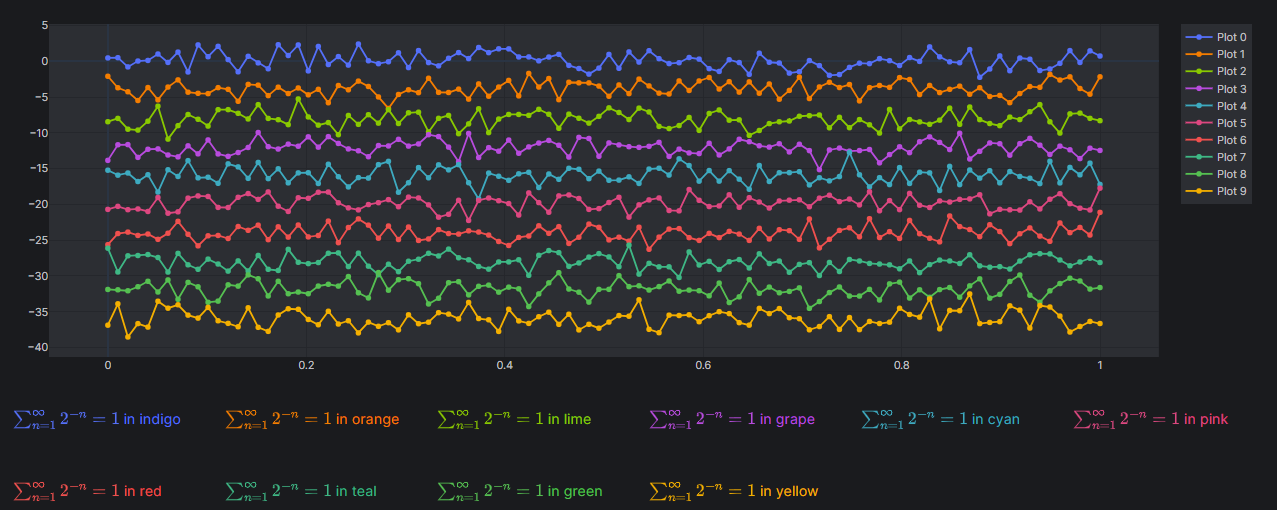
\includegraphics[width=\textwidth]{figures/gui/colors.png}
    \caption{Color matching between Plotly and Mantine}
    \label{fig:color_matching}
\end{figure}